\documentclass[10pt,a4paper]{article}
\usepackage{a4wide}
\usepackage[hyperfootnotes=false]{hyperref}
\usepackage{xcolor}
\usepackage{graphicx}


\renewcommand{\vec}[1]{\mathbf{#1}}
\newcommand{\lecture}{AutoML}
\newcommand{\lecturelong}{Automated Machine Learning}
\newcommand{\semester}{SS 2021}
\newcommand{\assignment}[1]{\nth{#1} Assignment}
\newcommand{\lectors}{M. Lindauer \& F. Hutter}
\newcommand{\hide}[1]{}


\newcommand{\gccs}{\paragraph{General constraints for code submissions}
{
\footnotesize{
Please adhere to these rules to make our and your life easier! We will deduct points if your solution does not fulfill the following:
    
    \begin{itemize}
    	\item If not stated otherwise, we will use exclusively Python $3.6$.
        \item If not stated otherwise, we expect a Python script, which we will invoke exactly as stated on the exercise sheet.
        \item Your solution exactly returns the required output (neither less nor more) -- you can implement a \texttt{--verbose} option to increase the verbosity level for developing.
        \item Add comments and docstrings, so we can understand your solution.
        \item (If applicable) The \texttt{README} describes how to install requirements or provides addition information.
        \item (If applicable) Add required additional packages to \texttt{requirements.txt}. Explain in your \texttt{README} what this package does, why you use that package and provide a link to it's documentation or GitHub page.
        \item (If applicable) All prepared unittests have to pass.
        \item (If applicable) You can (and sometimes have to) reuse code from previous exercises.
    \end{itemize}
    \rule{\textwidth}{.5pt}
    \smallskip\\
    \noindent}}}



\newcommand{\duedate}{September 13th 2021}
\newcommand{\due}{{\bf This project is due on \duedate.} }

\usepackage{fancyhdr}
\pagestyle{fancy}

\fancyhf{}
\lhead{Due: \duedate}
\chead{{\bf AutoML}\\Final Project}
\rhead{\lectors\\ \semester}
\cfoot{Page \thepage}

\begin{document}
	\paragraph{The final project} is part of the oral exam, which means you are \textbf{not allowed to work in groups}.
	The purpose of this project is for you to you get hands-on experience on most topics of the course and to show that you can present and explain the results of your work. 
	To get access to the template please use the following github classroom link\\ \url{https://classroom.github.com/a/dRo0fptr}.\footnote{This template prohibits groups.}

	The first $15$ minutes of the oral exam will be about your project. You will first present your approach and the results, and then we will discuss these together.
%	It is important that \textit{your evaluation builds the basis for discussion and \textbf{scientifically analyzes} which are the important aspects and characteristics of your approach}---you should present your findings in a convincing manner.
	To give the project presentation some structure, you will have to prepare a few slides.
	Your slides should consist of a motivation slide, slides detailing your approach (2-3) as well as slides for your results (2-3).
	%You are allowed to submit at most \textbf{5 slides}.
	\textit{Don't go overboard with your slides.}
	They are intended to make your presentation coherent, but your presentation should only be \textbf{7-8 minutes} to still have some time for discussions. %After 10 minutes we will have a hard cutoff if you are still presenting.
	It is important that \textit{your evaluation builds the basis for discussion and \textbf{scientifically analyzes} which are the important aspects and characteristics of your approach}---you should present your findings in a convincing manner.
	
	\section*{Optimization of a Convolutional Neural Network}
		
		Your task is to automatically improve and analyze the performance of a neural network for a \emph{flower classification}\footnote{\url{http://www.robots.ox.ac.uk/~vgg/data/flowers/17/index.html}} dataset.
		How you improve the performance of the given network is up to you \textbf{as long as it is by means of AutoML}. In addition, let us assume that you would like to deploy your model to a system with some hardware constraints (e.g. model size) or the application has some further fine-grained constraints on precision (e.g., in a medical application). Therefore, your AutoML system has to also adhere to constraints provided by users.
		
		
		%For example, you could optimize the hyperparameters of the network optimizer, apply neural architecture search or a joint approach.
		In the end, you should convince us that you indeed improved the performance of the network when compared to the default approach.
		To this end, you could consider one or several of the following:
		\begin{itemize}
			\item Apply HPO to obtain a well-performing hyperparameter configuration (e.g., BO or EAs);
			\item Apply NAS (e.g., BOHB or DARTS) to improve the architecture of the network;
			\item Extend the configuration space to cover preprocessing, data augmentation and regularization;
			\item Apply one or several of the speedup techniques for HPO/NAS;
			\item Apply multi-objective optimization;
			\item Apply meta-learning, such as algorithm selection or warmstarting, to improve the performance;
			\item Apply a learning to learn approach to learn how to optimize the network;
     		\item Determine the importance of the algorithm's hyperparameters;
		\end{itemize}
		\noindent
		Please note that you do not have to apply all of these methods -- pick the ones that you think are most appropriate.
		To evaluate your approach please choose the way you evaluate well; you could consider the following:
		\begin{itemize}
			\item Measure and compare against the default performance of the given network;
			\item Plot a confusion matrix;
			\item Plot the performance of your AutoML approach over time;
			\item Apply a statistical test.
		\end{itemize}

		\newpage
		\noindent		
		You are allowed to use all scripts and tools you already know from the exercises; however, you are not limited to them.
		Overall, you should respect the following constraints:
		\begin{itemize}
			\item \textbf{Metric:}
			\begin{itemize}
				\item The final performance has to be measured in terms of top-3 classification accuracy on a validation set.
				\textbf{However, your found configurations have to satisfy some constraints, such as, e.g. have a maximal network size of $2\cdot 10^7$ and a precision of at least $0.39$ (at least on validation set).}
				%\item Essentially, you are tasked with trying to find small networks with high accuracy.
				%\item To this end, show that your model lies on the pareto-front.
			\end{itemize}
			\item \textbf{Experimental Constraints:}
			\begin{itemize}
				\item Your code for making design decisions should run no longer than $86\,400$ seconds (without additional validation) on a single machine.
				\item Training a network can take at most 50 epochs.
				\item You can use any kind of hardware that is available to you. For example, you could also consider using Google Colab (which repeatedly offers a VM with a GPU for at most 12h for free) or Amazon SageMaker (which offers quite some resources for free if you are a first-time customer). \textit{Don't forget to state in your slides what kind of hardware you used!}
%				\item You can use at most 4 GPUs on the provided remote machines with at most $\frac{86\,400}{4}$ seconds per GPU\footnote{We provide access to Nvidia Titan Black GPUs via our SLURM schedule system. Please note that you don't have exclusive access to them and we strongly recommend to start with the project early on. We explicitly emphasize that it is not a valid excuse to say that you got no GPU time the very last days before the deadline.}.
			\end{itemize}
			\item \textbf{Implementation Constraints:}
			\begin{itemize}
			  \item You can freely extend the baseline implementation provided to you. However, your search space should always include the given default network.
			  \item You are not allowed to use manual tuning to achieve better performance. All improved design decisions have to be made (somehow) automatically.
			  \item You need to provide a script ``AutoML.py'' running your optimizer that accepts at least the following arguments:\\
			  \texttt{--constraint\_max\_model\_size [int]}\\
			  \texttt{--constraint\_min\_precision [float]}
			\end{itemize}
			\item \textbf{Grading Guidelines:}
			\begin{itemize}
			  \item We grade your projects based on: sound motivation for the chosen approach, achieved performance, convincing presentation, scientific workflow, reproducible results and answers to our questions.
			  \item We expect that you find at least a configuration that has a top-3 accuracy $\geq 0.8$.
			  \item To earn a 2.0 as a grade, we expect at least that:
			  \begin{itemize}
			  	\item You apply the correct approaches and tools you learned about in the lecture.
			  	\item Your approach does not violate different constraints on network sizes\\ (in particular, $2\cdot10^7, 5\cdot10^7, 1\cdot10^8$).\footnote{If these constraints are too easy for your implementations, you can also use harder constraints (i.e., constraints on small network sizes). In any case, we might assess your submission with other network sizes as constraints.}
			  \end{itemize}
			  \item To earn a grade better than 2.0, we expect at least that:
			  \begin{itemize}
			  	\item You have your own ideas on how to improve an approach from the lectures. For example two years ago, a student combined hyperparameter importance and BOHB in an interesting way and showed that it improved the overall performance.
			  	\item Your found solutions adhere to the network size constraint and different constraints on minimal precision (in particular, $0.39$, $0.40$, $0.42$, at least on validation set).
			  \end{itemize}
			  \begin{figure}[t]
			  	\centering
			  	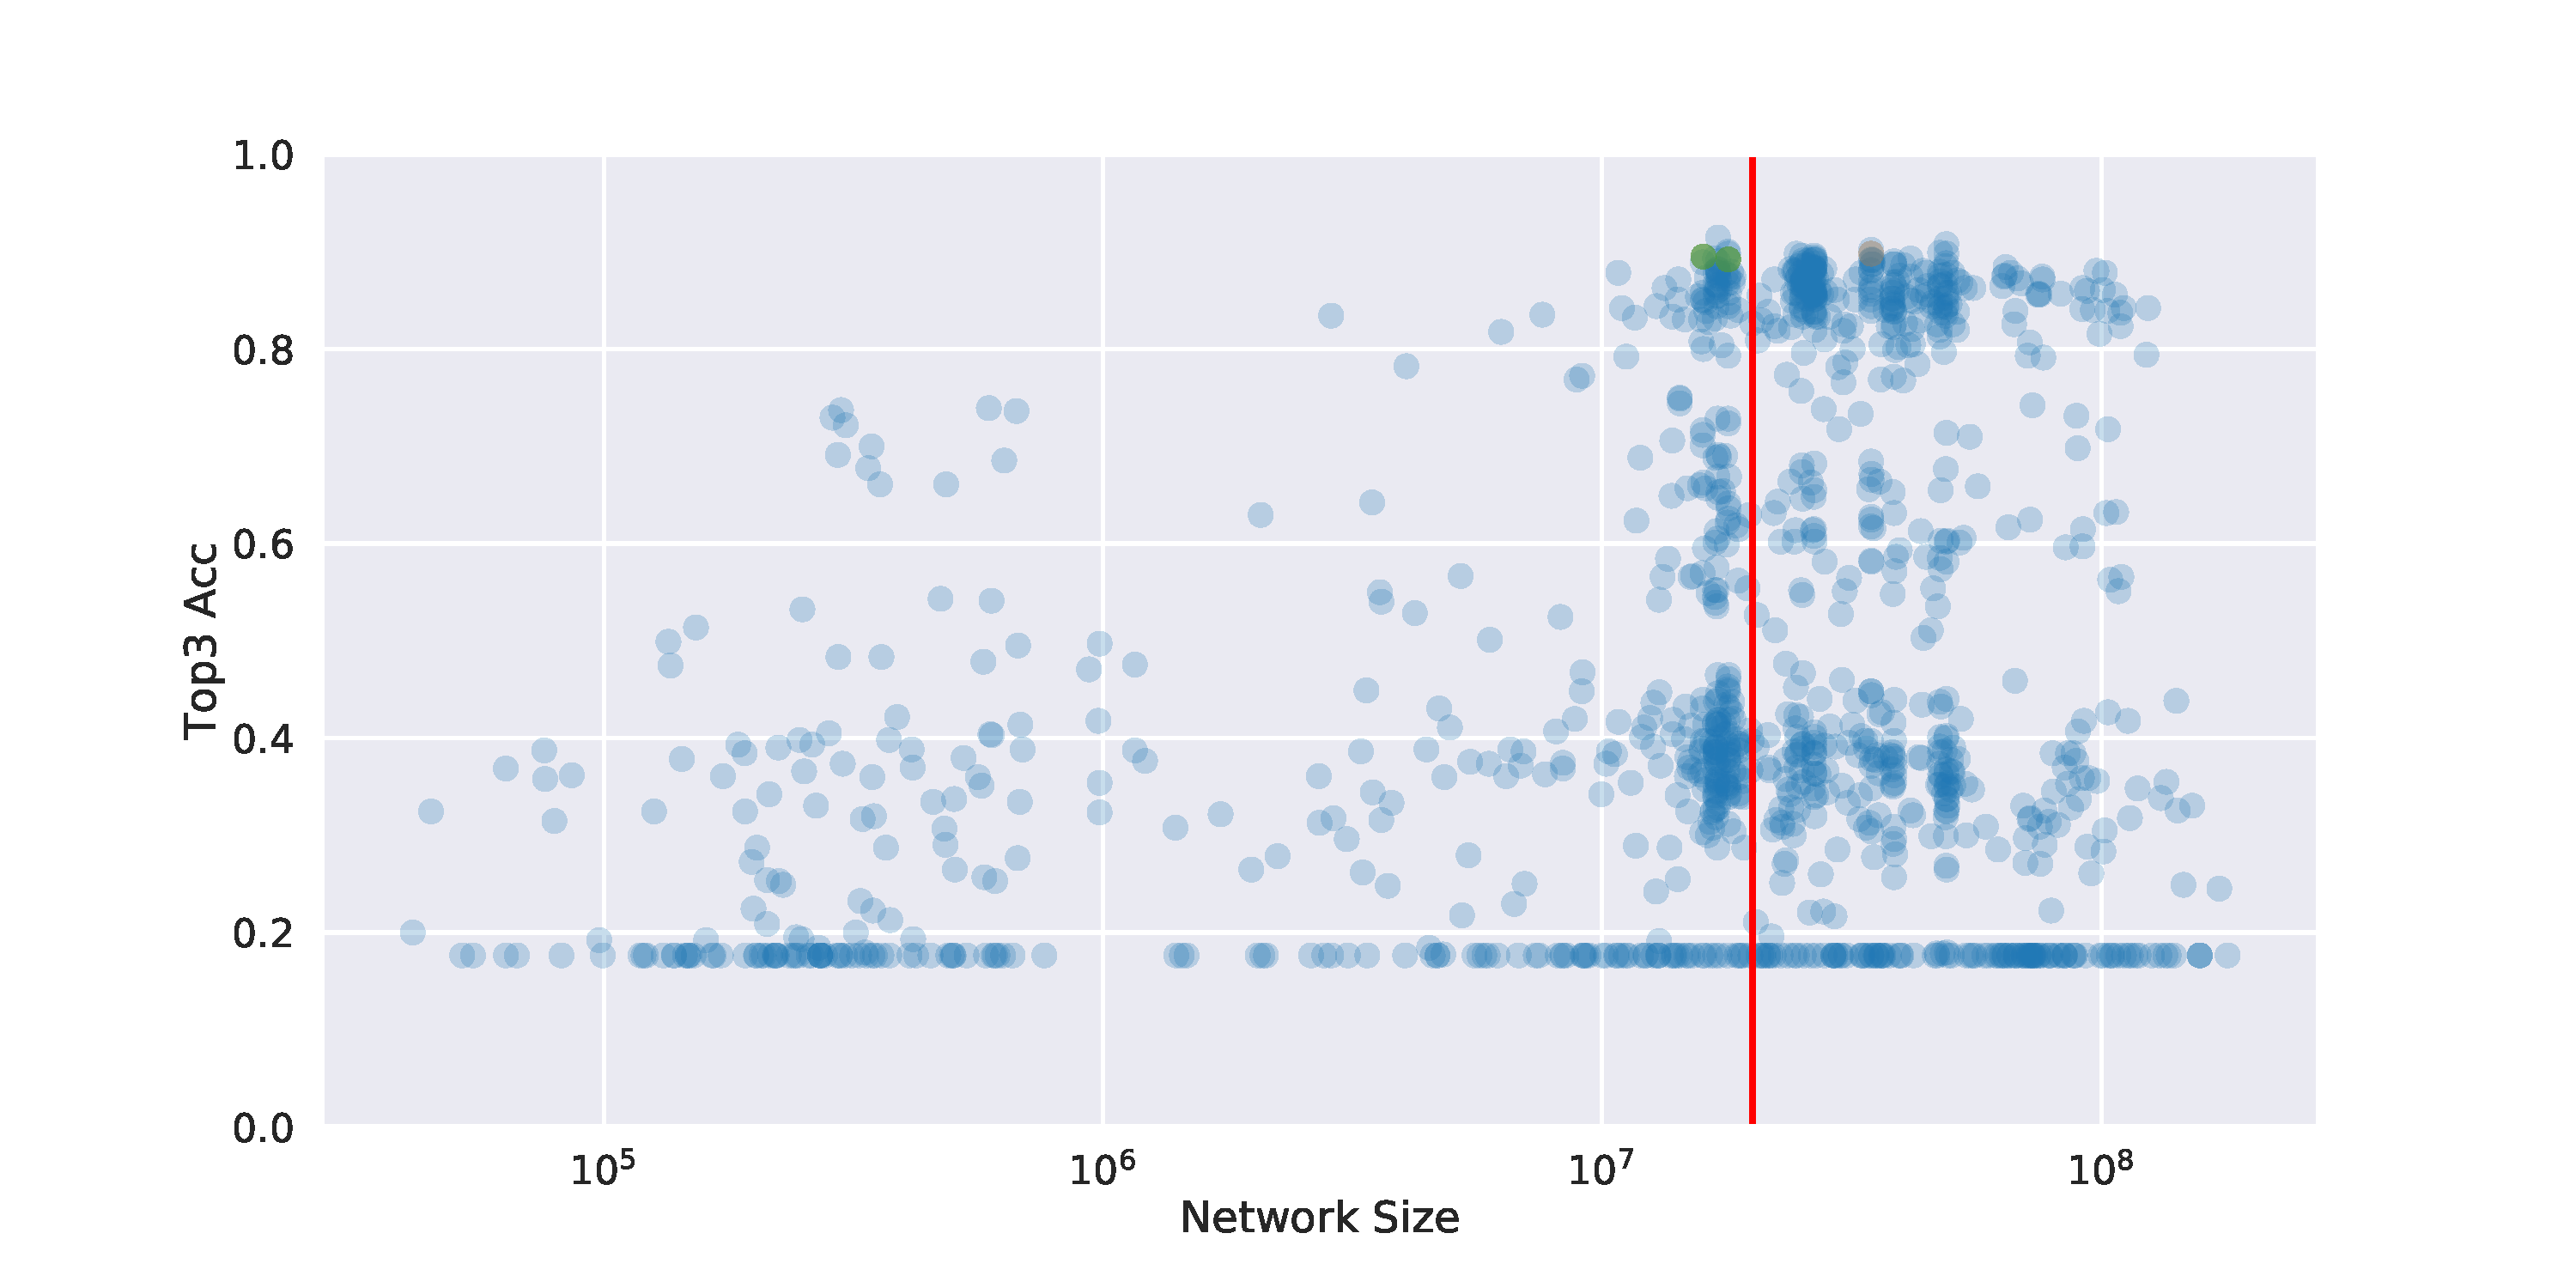
\includegraphics[width=1\textwidth]{baselines.pdf}
			  	\caption{Evaluated configurations on the configuration space with a configuration budget $10$ times larger than your allowed budget. The y-axis gives the top-3 accuracy in percent and the x-axis the network size in terms of the number of parameters of each model. The red line shows the network-size constraint of $2\cdot10^7$. Orange dots adhere only to the precision constraint of $0.39$. The green dots adhere to both constraints.}\label{fig1}
			  \end{figure}
			\end{itemize}
		\end{itemize}
		
		As a starting point, we provide  a repository containing:
		\begin{itemize}
			\item A cropped and downsized version of the original flower classification dataset. The images are only of size $16\times16$.
			\item A default parameterized network to optimize (written in pytorch)
			\item An example script to show you how to train and evaluate a network based on the default configuration
			\item An example script that shows you how to use BOHB in SMAC.
		\end{itemize}
		
		%ML: has not really worked in the past two years.
		%We provide a Google spreadsheet\footnote{\url{TODO}} in which you can upload your current progress. This sheet will not be monitored by us but gives you the opportunity to compare your results. This might help you identify early if your approach is working well or not.\\[1em]
		
%\vspace*{\fill}\\
\noindent
\due Students should submit their PDF for the presentation to \texttt{biedenka@cs.uni-freiburg.de} (Freiburg) / \texttt{deng@tnt.uni-hannover.de} (Hannover). \textbf{No teams are allowed for the final project.}
\end{document}

